\documentclass{beamer}
\usetheme{Madrid}
\usecolortheme{default}

\usepackage[utf8]{inputenc}
\usepackage[T5]{fontenc}
\usepackage[vietnamese,english]{babel}
\usepackage{amsmath}
\usepackage{amssymb}
\usepackage{graphicx}
\usepackage{algorithm}
\usepackage{algpseudocode}
\usepackage{tikz}
\usepackage{booktabs}
\usepackage{multirow}

\graphicspath{{figs/}}

\title{Credit Card Fraud Detection}
\subtitle{XGBoost, Chunk Evaluation \& Drift Analysis}
\author{Nguyen Huy Minh}
\institute{AI66A, National Economics University}
\date{April 29, 2026}

\setbeamertemplate{footline}{
  \leavevmode%
  \hbox{%
  \begin{beamercolorbox}[wd=.85\paperwidth,ht=2.25ex,dp=1ex,left,leftskip=3ex]{title in head/foot}%
    \usebeamerfont{title in head/foot}\insertshorttitle
  \end{beamercolorbox}%
  \begin{beamercolorbox}[wd=.15\paperwidth,ht=2.25ex,dp=1ex,right,rightskip=3ex]{title in head/foot}%
    \insertframenumber{} / \inserttotalframenumber
  \end{beamercolorbox}%
  }%
  \vskip0pt%
}

\begin{document}

% Title slide
\begin{frame}
    \titlepage
\end{frame}

\begin{frame}{Outline}
    \begin{columns}[onlytextwidth, c]
        \begin{column}{0.48\textwidth}
            \tableofcontents
        \end{column}
        \begin{column}{0.5\textwidth}
            \begin{center}
                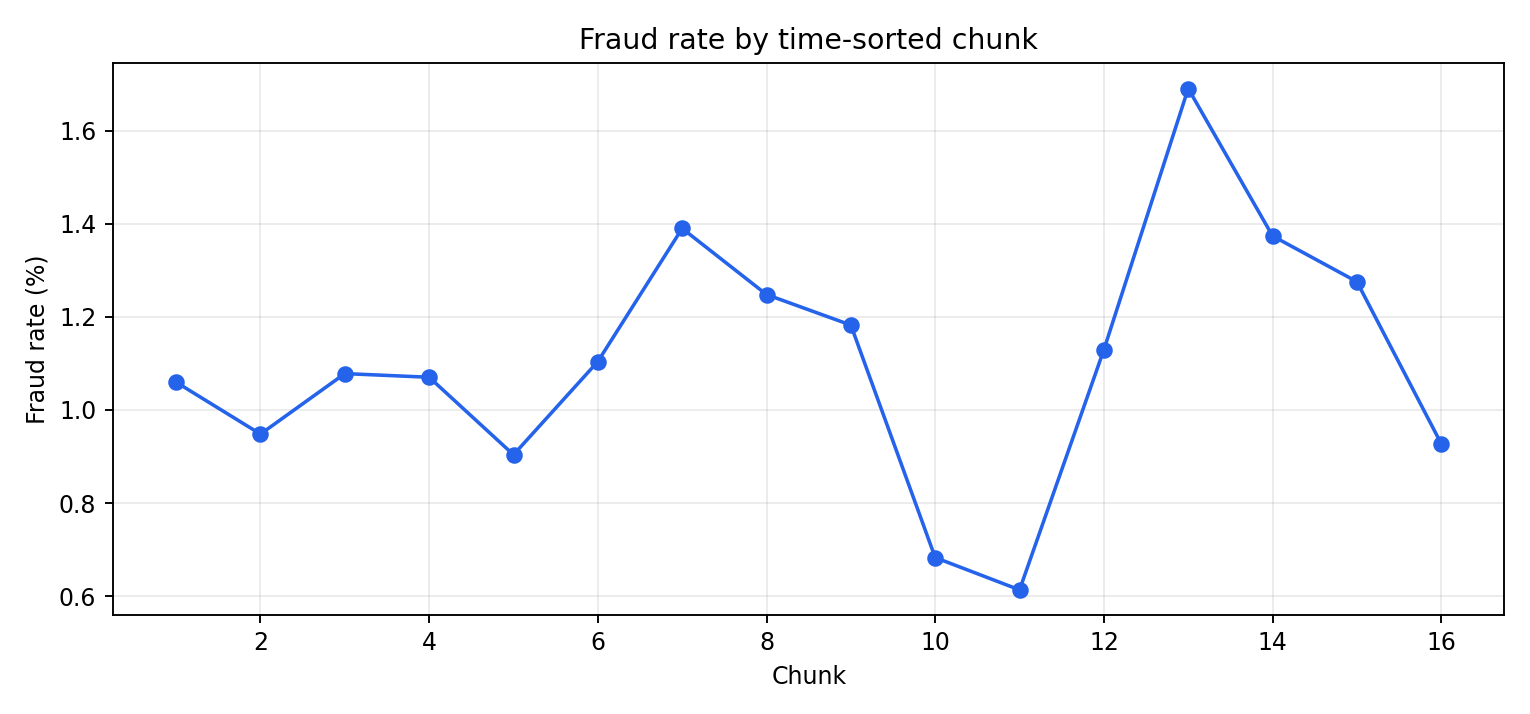
\includegraphics[width=\textwidth]{fraud_rate_by_chunk.png}

                \vspace{0.3cm}

                \small
                \textit{Figure: Fraud rate by time-sorted chunk}
            \end{center}
        \end{column}
    \end{columns}
\end{frame}

\section{Problem Statement}

\begin{frame}{Problem Statement}
    \textbf{Challenge}: Fraud detection is an imbalanced classification problem where fraudulent transactions are rare but high-impact.

    \vspace{0.45cm}
    \textbf{Key issues}:
    \begin{itemize}
        \item Accuracy is misleading because the non-fraud class dominates.
        \item Fraud patterns can change over time, causing concept or distribution drift.
        \item A fixed threshold can become invalid even when model ranking remains good.
        \item False negatives lose fraud cases; false positives create unnecessary alerts.
    \end{itemize}

    \vspace{0.45cm}
    \textbf{Goal}: Build an XGBoost-based fraud detector and evaluate whether low F1 scores are caused by concept drift or threshold/calibration drift.
\end{frame}

\section{Dataset and Features}

\begin{frame}{Dataset Overview}
    \textbf{Dataset}: Time-sorted credit card transaction data split into 16 parquet chunks.

    \vspace{0.35cm}
    \begin{table}
        \centering
        \small
        \begin{tabular}{l r}
            \toprule
            \textbf{Attribute} & \textbf{Value} \\
            \midrule
            Total transactions & 8,580,255 \\
            Fraud transactions & 94,806 \\
            Overall fraud rate & 1.105\% \\
            Number of chunks & 16 \\
            Rows per chunk & $\approx$ 536K \\
            Evaluated chunks & 02--16 \\
            \bottomrule
        \end{tabular}
    \end{table}

    \vspace{0.25cm}
    \textbf{Note}: Chunk 16 has no fraud cases in the test segment, so it is excluded from model-quality conclusions.
\end{frame}

\begin{frame}{Fraud Rate Over Time}
    \begin{figure}
        \centering
        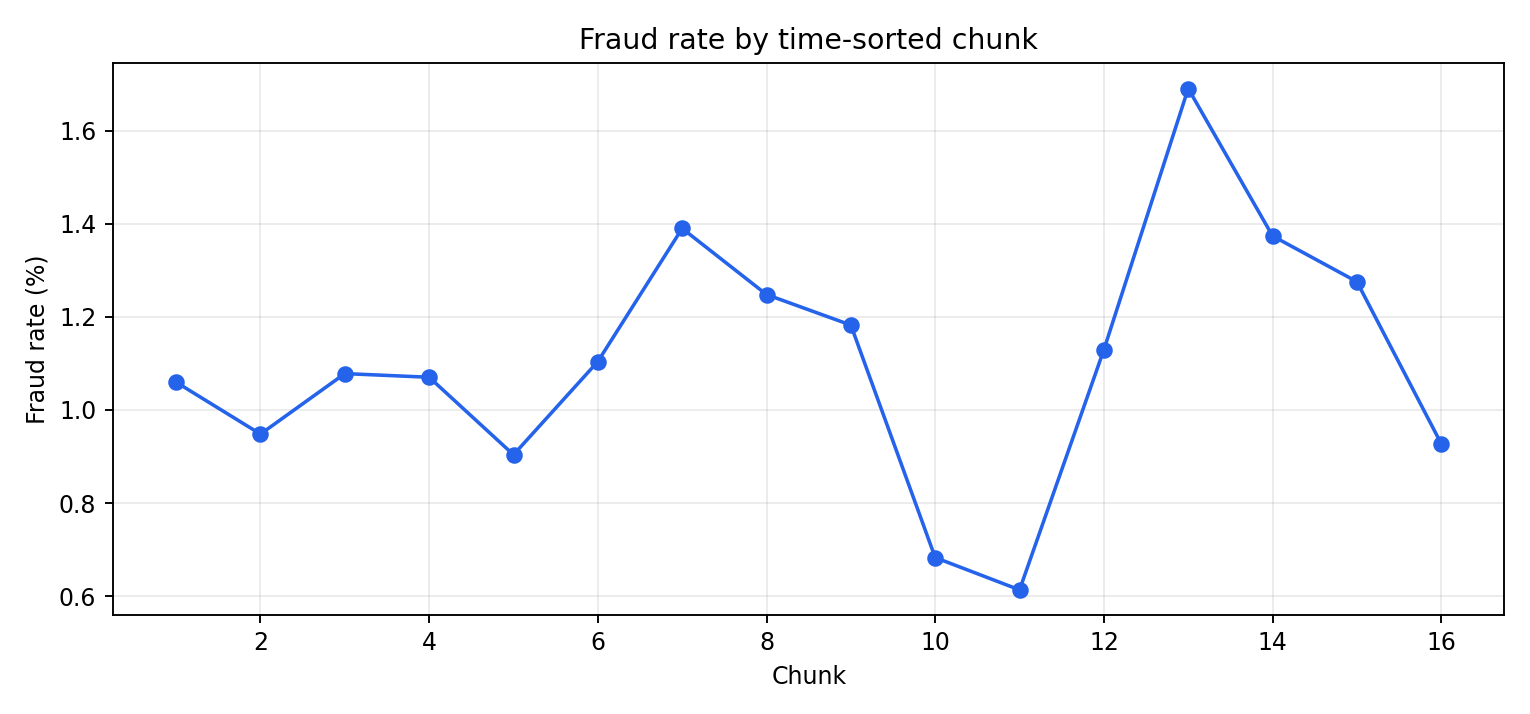
\includegraphics[width=0.88\textwidth]{fraud_rate_by_chunk.png}
        \caption{Fraud rate varies across time-sorted chunks, indicating possible prior or distribution shift.}
    \end{figure}
\end{frame}

\section{EDA on Data Chunk 01}

\begin{frame}{Chunk 01: Data Quality Overview}
    \textbf{Source used in notebook}: \texttt{data\_chunks\_16/transactions\_time\_sorted\_part\_01.parquet}

    \vspace{0.25cm}
    \begin{table}
        \centering
        \small
        \begin{tabular}{l r}
            \toprule
            \textbf{Attribute} & \textbf{Value} \\
            \midrule
            Rows & 536,266 \\
            Columns & 44 \\
            Missing values & 0 across all columns \\
            Unique transactions & 536,266 \\
            Unique cards/accounts & 8,757 \\
            Categories & 14 \\
            Merchants & 655 \\
            Jobs & 639 \\
            Transaction period & 2022-05-06 23:00:01 to 2022-05-30 02:24:20 \\
            \bottomrule
        \end{tabular}
    \end{table}

    \vspace{0.15cm}
    \textbf{EDA implication}: data is clean enough for modeling, but high-cardinality categorical variables require encoding.
\end{frame}

\begin{frame}{Chunk 01: Target Imbalance}
    \begin{columns}[onlytextwidth, c]
        \begin{column}{0.48\textwidth}
            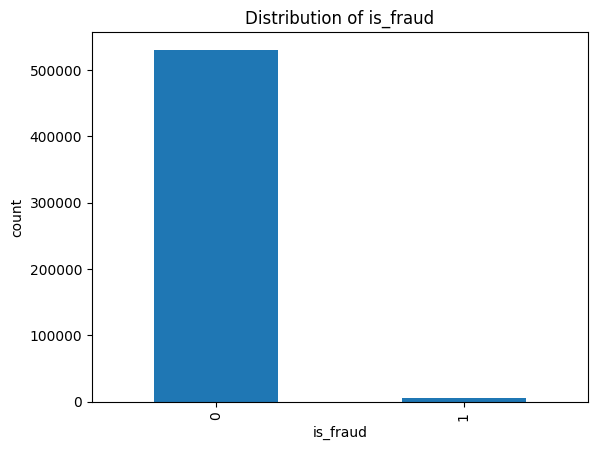
\includegraphics[width=\textwidth]{notebook/cell_16_img_01.png}
        \end{column}
        \begin{column}{0.5\textwidth}
            \begin{table}
                \centering
                \small
                \begin{tabular}{lrr}
                    \toprule
                    \textbf{Class} & \textbf{Count} & \textbf{Rate} \\
                    \midrule
                    Non-fraud & 530,583 & 98.9403\% \\
                    Fraud & 5,683 & 1.0597\% \\
                    \bottomrule
                \end{tabular}
            \end{table}

            \vspace{0.2cm}
            \begin{itemize}
                \item Accuracy is not a meaningful metric.
                \item PR-AUC, recall, precision, and F1 are more useful.
                \item XGBoost needs imbalance handling through class weight or undersampling.
            \end{itemize}
        \end{column}
    \end{columns}
\end{frame}

\begin{frame}{Chunk 01: Datetime and Age}
    \begin{table}
        \centering
        \small
        \begin{tabular}{lrr}
            \toprule
            \textbf{Variable} & \textbf{Minimum} & \textbf{Maximum} \\
            \midrule
            Date of birth & 1927-07-06 & 2008-07-03 \\
            Transaction datetime & 2022-05-06 23:00:01 & 2022-05-30 02:24:20 \\
            Age & 14 & 95 \\
            \bottomrule
        \end{tabular}
    \end{table}

    \vspace{0.25cm}
    \begin{table}
        \centering
        \small
        \begin{tabular}{lrrrrr}
            \toprule
            \textbf{Age statistic} & \textbf{Mean} & \textbf{Std} & \textbf{Q1} & \textbf{Median} & \textbf{Q3} \\
            \midrule
            Age & 44.23 & 17.90 & 30 & 41 & 55 \\
            \bottomrule
        \end{tabular}
    \end{table}

    \vspace{0.15cm}
    \textbf{Feature decision}: use ordinal \texttt{age\_bin\_ord} instead of raw age to capture non-linear age-group effects.
\end{frame}

\begin{frame}{Time EDA: Hour of Day}
    \begin{figure}
        \centering
        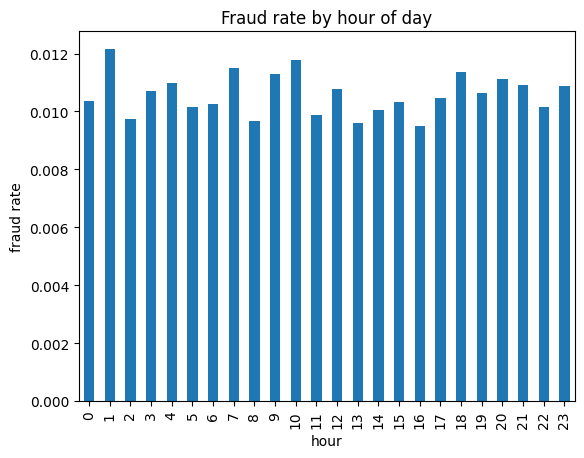
\includegraphics[width=0.78\textwidth]{notebook/cell_23_img_01.png}
        \caption{Fraud rate by transaction hour in chunk 01.}
    \end{figure}

    \vspace{-0.15cm}
    \small
    \textbf{Insight}: fraud is spread relatively evenly by hour. Night indicator alone is weak because fraud and non-fraud have very similar night rates.
\end{frame}

\begin{frame}{Time EDA: Weekday vs Weekend}
    \begin{table}
        \centering
        \small
        \begin{tabular}{lrrr}
            \toprule
            \textbf{Segment} & \textbf{Total} & \textbf{Fraud} & \textbf{Fraud rate} \\
            \midrule
            Weekday & 285,937 & 3,778 & 1.3213\% \\
            Weekend & 250,329 & 1,905 & 0.7610\% \\
            \bottomrule
        \end{tabular}
    \end{table}

    \vspace{0.3cm}
    \begin{itemize}
        \item Fraud appears more often on weekdays in chunk 01.
        \item This contradicts a simple rule such as ``fraud happens mostly at night/weekend''.
        \item \texttt{trans\_date\_is\_weekend} is still useful, but the direction should be learned by the model.
    \end{itemize}
\end{frame}

\begin{frame}{Time EDA: Month and Age Group}
    \begin{columns}[onlytextwidth, c]
        \begin{column}{0.49\textwidth}
            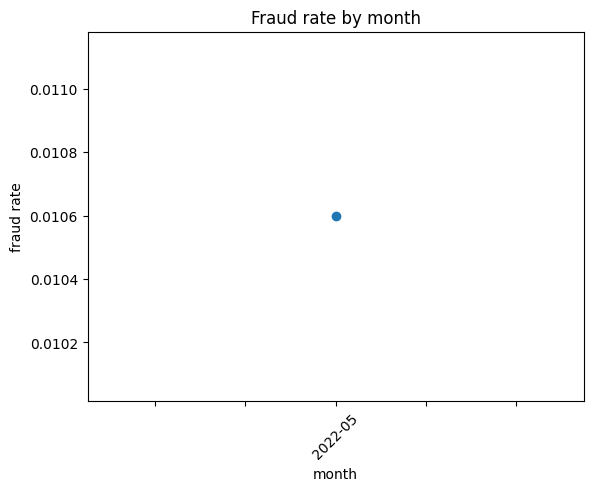
\includegraphics[width=\textwidth]{notebook/cell_27_img_01.png}
            \centering
            \scriptsize Month-level fraud rate
        \end{column}
        \begin{column}{0.49\textwidth}
            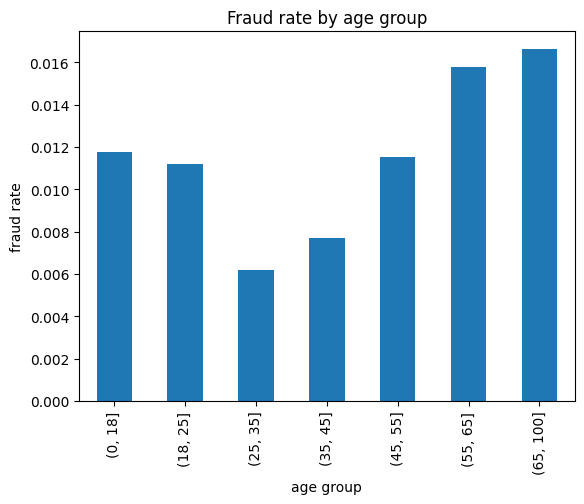
\includegraphics[width=\textwidth]{notebook/cell_29_img_01.png}
            \centering
            \scriptsize Fraud rate by age bin
        \end{column}
    \end{columns}

    \vspace{0.25cm}
    \small
    Older age groups show higher fraud rates in this chunk: age 55--65 has 1.58\%, age 65--100 has 1.66\%.
\end{frame}

\begin{frame}{Categorical EDA: Cardinality}
    \begin{table}
        \centering
        \small
        \begin{tabular}{lrrrr}
            \toprule
            \textbf{Column} & \textbf{Type} & \textbf{Unique} & \textbf{Null count} & \textbf{Null rate} \\
            \midrule
            merchant & string & 655 & 0 & 0.0\% \\
            job & string & 639 & 0 & 0.0\% \\
            category & string & 14 & 0 & 0.0\% \\
            gender & string & 2 & 0 & 0.0\% \\
            \bottomrule
        \end{tabular}
    \end{table}

    \vspace{0.35cm}
    \textbf{Encoding decision}:
    \begin{itemize}
        \item \texttt{category}: one-hot encoding because cardinality is low.
        \item \texttt{merchant}, \texttt{job}: frequency encoding because cardinality is high.
        \item \texttt{gender}: binary encoding.
    \end{itemize}
\end{frame}

\begin{frame}{Categorical EDA: Category and Gender}
    \begin{columns}[onlytextwidth, c]
        \begin{column}{0.58\textwidth}
            \begin{table}
                \centering
                \tiny
                \begin{tabular}{lrrr}
                    \toprule
                    \textbf{Category} & \textbf{Total} & \textbf{Fraud} & \textbf{Rate} \\
                    \midrule
                    grocery\_pos & 1,394 & 1,394 & 100.0\% \\
                    shopping\_net & 1,299 & 1,299 & 100.0\% \\
                    misc\_net & 744 & 744 & 100.0\% \\
                    shopping\_pos & 659 & 659 & 100.0\% \\
                    gas\_transport & 458,338 & 465 & 0.1015\% \\
                    grocery\_net & 72,804 & 94 & 0.1291\% \\
                    \bottomrule
                \end{tabular}
            \end{table}
        \end{column}
        \begin{column}{0.4\textwidth}
            \begin{table}
                \centering
                \scriptsize
                \begin{tabular}{lrrr}
                    \toprule
                    \textbf{Gender} & \textbf{Total} & \textbf{Fraud} & \textbf{Rate} \\
                    \midrule
                    M & 266,428 & 2,963 & 1.112\% \\
                    F & 269,838 & 2,720 & 1.008\% \\
                    \bottomrule
                \end{tabular}
            \end{table}
        \end{column}
    \end{columns}

    \vspace{0.2cm}
    \small
    \textbf{Warning}: several categories are almost deterministic in chunk 01, so metrics must be checked across future chunks to avoid over-trusting category artifacts.
\end{frame}

\begin{frame}{Categorical EDA: Merchant and Job}
    \begin{columns}[onlytextwidth, t]
        \begin{column}{0.48\textwidth}
            \textbf{Merchant signal}
            \begin{itemize}
                \item Top fraud merchant rates are only around 0.2--0.3\%.
                \item Merchant alone is weaker than category.
                \item Frequency encoding is kept as a compact signal.
            \end{itemize}
        \end{column}
        \begin{column}{0.5\textwidth}
            \textbf{Top job fraud rates}
            \begin{table}
                \centering
                \tiny
                \begin{tabular}{lr}
                    \toprule
                    \textbf{Job} & \textbf{Fraud rate} \\
                    \midrule
                    Scientist, product/process dev. & 9.82\% \\
                    Systems developer & 7.00\% \\
                    Theatre manager & 6.38\% \\
                    Copywriter, advertising & 5.99\% \\
                    Holiday representative & 5.42\% \\
                    \bottomrule
                \end{tabular}
            \end{table}
        \end{column}
    \end{columns}

    \vspace{0.2cm}
    \textbf{Insight}: job has stronger discriminative signal than merchant in chunk 01.
\end{frame}

\begin{frame}{Numeric EDA: Fraud vs Non-Fraud}
    \begin{table}
        \centering
        \scriptsize
        \begin{tabular}{lrrrr}
            \toprule
            \textbf{Feature} & \textbf{Non-fraud mean} & \textbf{Fraud mean} & \textbf{Non-fraud median} & \textbf{Fraud median} \\
            \midrule
            amt & 78.57 & 534.61 & 61.51 & 389.44 \\
            trans\_time\_hrs & 11.50 & 11.48 & 12.00 & 11.00 \\
            trans\_date\_is\_weekend & 0.468 & 0.335 & 0.00 & 0.00 \\
            merchant\_risk\_30\_day & 16.12 & 16.25 & 17.00 & 17.00 \\
            customer\_num\_trans\_30\_day & 13.00 & 13.04 & 13.00 & 13.00 \\
            \bottomrule
        \end{tabular}
    \end{table}

    \vspace{0.25cm}
    \begin{itemize}
        \item Amount is the strongest numeric signal: fraud mean is about 6.8x non-fraud mean.
        \item Rolling customer/merchant counts have much weaker univariate separation.
    \end{itemize}
\end{frame}

\begin{frame}{Numeric Distributions I}
    \begin{columns}[onlytextwidth]
        \begin{column}{0.5\textwidth}
            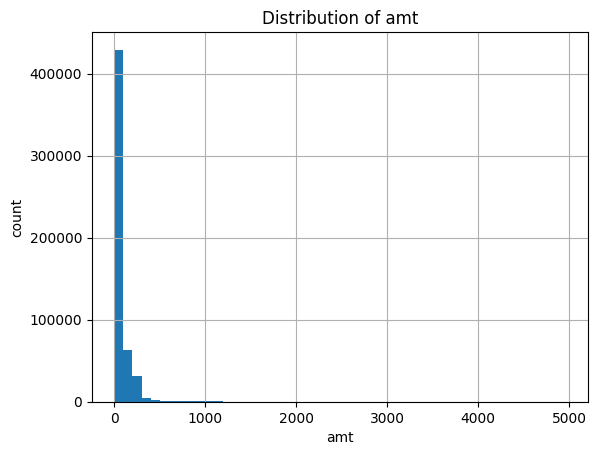
\includegraphics[width=\textwidth]{notebook/cell_44_img_01.png}
            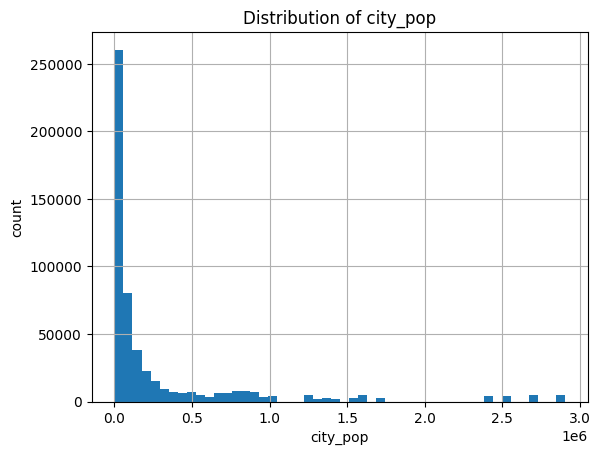
\includegraphics[width=\textwidth]{notebook/cell_44_img_02.png}
        \end{column}
        \begin{column}{0.5\textwidth}
            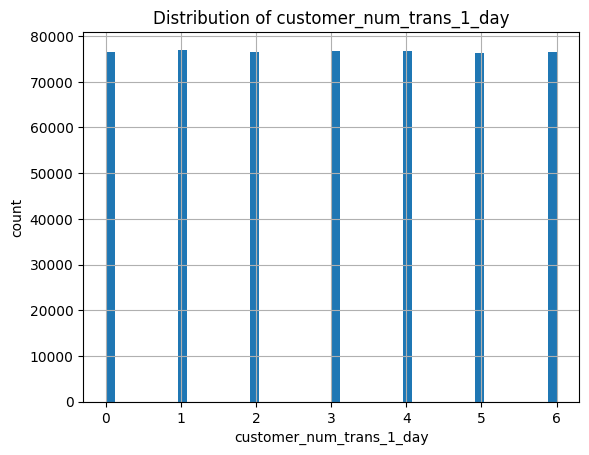
\includegraphics[width=\textwidth]{notebook/cell_44_img_03.png}
            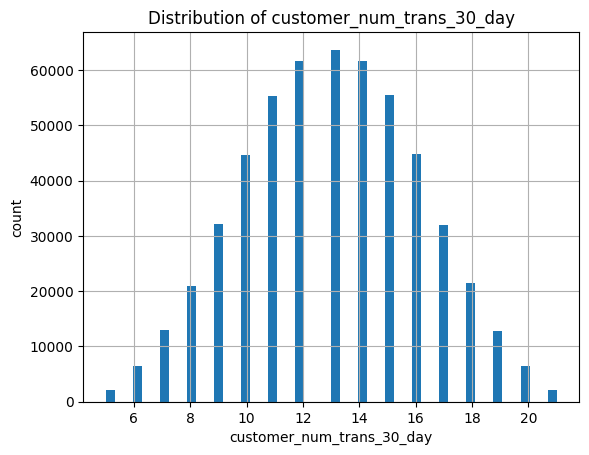
\includegraphics[width=\textwidth]{notebook/cell_44_img_04.png}
        \end{column}
    \end{columns}
\end{frame}

\begin{frame}{Numeric Distributions II}
    \begin{columns}[onlytextwidth]
        \begin{column}{0.33\textwidth}
            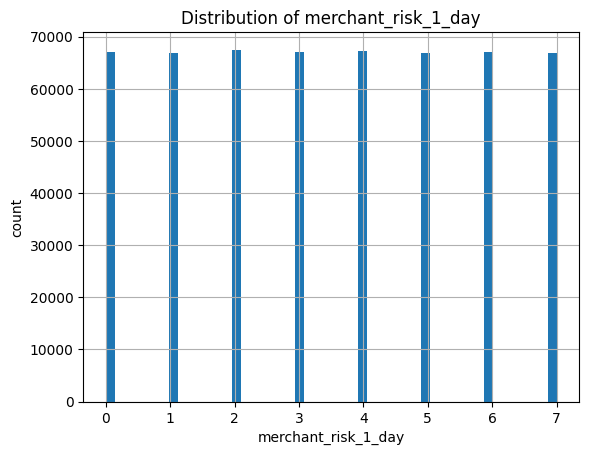
\includegraphics[width=\textwidth]{notebook/cell_44_img_05.png}
        \end{column}
        \begin{column}{0.33\textwidth}
            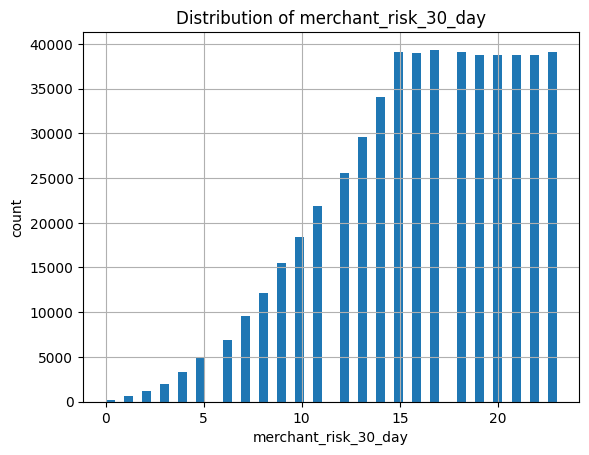
\includegraphics[width=\textwidth]{notebook/cell_44_img_06.png}
        \end{column}
        \begin{column}{0.33\textwidth}
            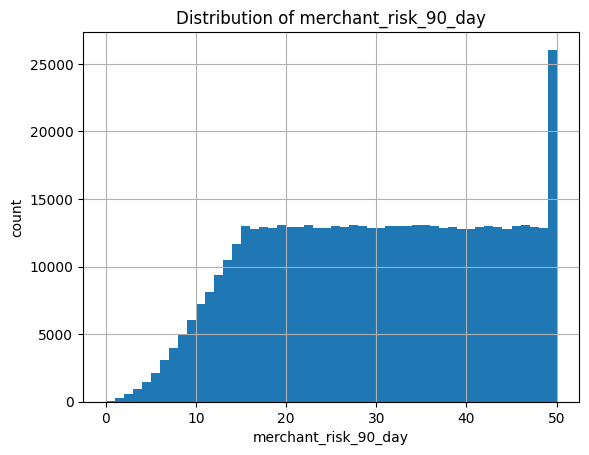
\includegraphics[width=\textwidth]{notebook/cell_44_img_07.png}
        \end{column}
    \end{columns}

    \vspace{0.25cm}
    \small
    Merchant risk features are retained for interactions, although their univariate separation is weak.
\end{frame}

\begin{frame}{Boxplots by Target}
    \begin{columns}[onlytextwidth]
        \begin{column}{0.33\textwidth}
            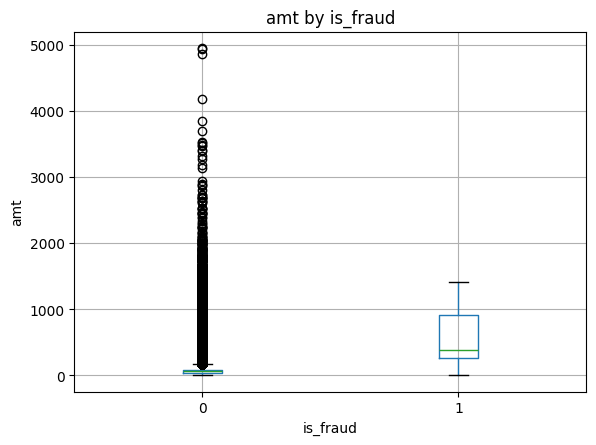
\includegraphics[width=\textwidth]{notebook/cell_46_img_01.png}
            \centering
            \scriptsize \texttt{amt}
        \end{column}
        \begin{column}{0.33\textwidth}
            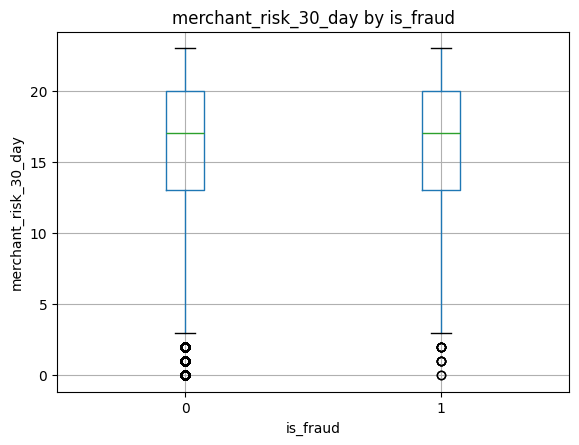
\includegraphics[width=\textwidth]{notebook/cell_46_img_02.png}
            \centering
            \scriptsize \texttt{merchant\_risk\_30\_day}
        \end{column}
        \begin{column}{0.33\textwidth}
            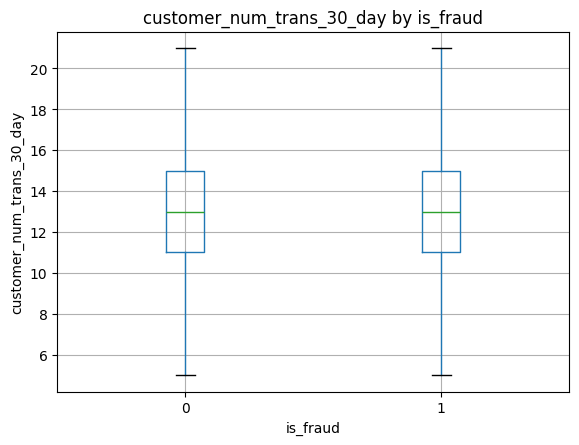
\includegraphics[width=\textwidth]{notebook/cell_46_img_03.png}
            \centering
            \scriptsize \texttt{customer\_num\_trans\_30\_day}
        \end{column}
    \end{columns}
\end{frame}

\begin{frame}{Correlation with Target}
    \begin{figure}
        \centering
        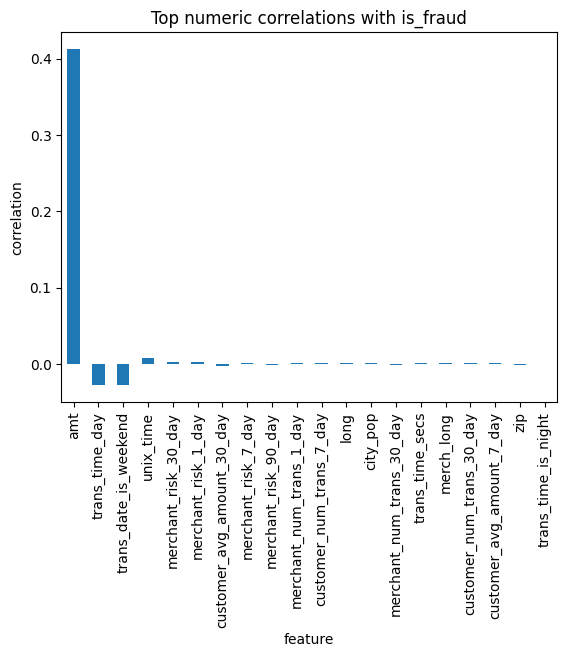
\includegraphics[width=0.82\textwidth]{notebook/cell_48_img_01.png}
        \caption{Top numeric correlations with \texttt{is\_fraud}.}
    \end{figure}

    \vspace{-0.15cm}
    \small
    Linear correlation is useful for screening, but tree-based models can exploit non-linear splits and interactions.
\end{frame}

\begin{frame}{Geographic EDA: Customer--Merchant Distance}
    \begin{columns}[onlytextwidth, c]
        \begin{column}{0.48\textwidth}
            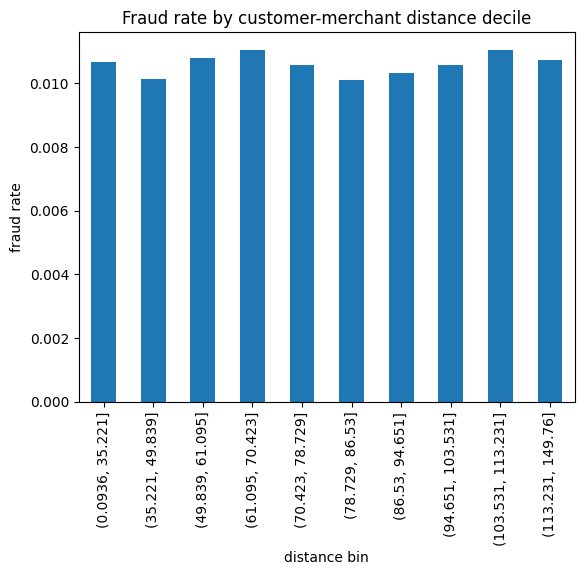
\includegraphics[width=\textwidth]{notebook/cell_51_img_01.png}
        \end{column}
        \begin{column}{0.5\textwidth}
            \begin{table}
                \centering
                \scriptsize
                \begin{tabular}{lrr}
                    \toprule
                    \textbf{Class} & \textbf{Mean km} & \textbf{Median km} \\
                    \midrule
                    Non-fraud & 76.55 & 78.73 \\
                    Fraud & 76.77 & 78.60 \\
                    \bottomrule
                \end{tabular}
            \end{table}

            \vspace{0.25cm}
            \begin{itemize}
                \item Distance deciles are almost flat.
                \item Difference between fraud and non-fraud distance is negligible.
                \item Decision: drop distance, merchant latitude and merchant longitude.
            \end{itemize}
        \end{column}
    \end{columns}
\end{frame}

\begin{frame}{EDA Summary for Chunk 01}
    \textbf{Main findings from notebook outputs}:
    \begin{itemize}
        \item Severe class imbalance: fraud rate is only 1.0597\%.
        \item Amount is the strongest numeric signal.
        \item Some categories are near-deterministic in chunk 01, so cross-chunk validation is required.
        \item Time-of-day is weak; weekday/weekend has more visible signal.
        \item Job has stronger signal than merchant; merchant alone is weak.
        \item Customer--merchant distance is not useful in this dataset.
    \end{itemize}

    \vspace{0.25cm}
    \textbf{Modeling implication}: use PR-AUC/F1, class weighting, time-based split, and cross-chunk drift checks.
\end{frame}

\begin{frame}{Feature Engineering}
    \textbf{Final feature set}: 25 selected features used for XGBoost.

    \vspace{0.35cm}
    \begin{columns}
        \begin{column}{0.5\textwidth}
            \textbf{\textcolor{blue}{Feature groups}}
            \begin{itemize}
                \item Amount: \texttt{amt}, amount-vs-habit ratio
                \item Customer rolling behavior
                \item Merchant rolling risk
                \item Time indicators: day, weekend, night
                \item Frequency encodings for merchant and job
            \end{itemize}
        \end{column}
        \begin{column}{0.5\textwidth}
            \textbf{\textcolor{red}{Dropped or controlled}}
            \begin{itemize}
                \item ID-like columns: card/account/profile IDs
                \item Raw datetime columns after feature extraction
                \item \texttt{unix\_time}: only used for sorting
                \item High-cardinality raw text categories
            \end{itemize}
        \end{column}
    \end{columns}
\end{frame}

\begin{frame}{Leakage Control and Time Split}
    \textbf{Time-based evaluation protocol per chunk}:
    \begin{itemize}
        \item 64\% train-inner
        \item 16\% validation
        \item 20\% final test
    \end{itemize}

    \vspace{0.35cm}
    \textbf{Leakage controls}:
    \begin{itemize}
        \item Model never uses future rows for training.
        \item Threshold is selected on validation only.
        \item Test labels are used only for final reporting.
        \item \texttt{best\_test\_f1\_diagnostic} is diagnostic only, not a deployment threshold.
    \end{itemize}
\end{frame}

\section{Feature Selection}

\begin{frame}{Mutual Information Ranking}
    \begin{columns}[onlytextwidth, c]
        \begin{column}{0.52\textwidth}
            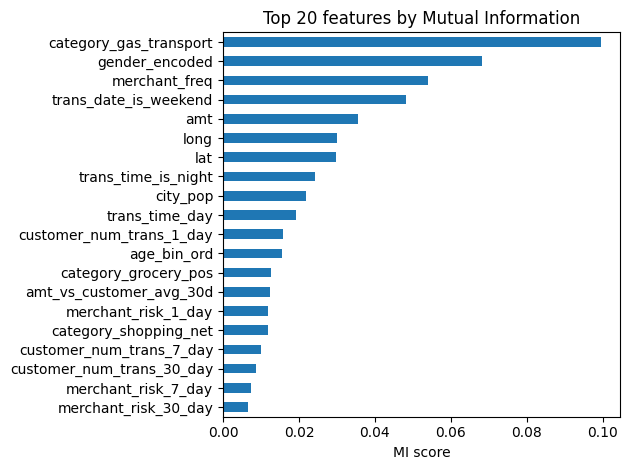
\includegraphics[width=\textwidth]{notebook/cell_60_img_01.png}
        \end{column}
        \begin{column}{0.46\textwidth}
            \textbf{Top MI signals}
            \begin{table}
                \centering
                \tiny
                \begin{tabular}{lr}
                    \toprule
                    \textbf{Feature} & \textbf{MI} \\
                    \midrule
                    category\_gas\_transport & 0.0995 \\
                    gender\_encoded & 0.0683 \\
                    merchant\_freq & 0.0540 \\
                    trans\_date\_is\_weekend & 0.0483 \\
                    amt & 0.0354 \\
                    long & 0.0300 \\
                    lat & 0.0297 \\
                    trans\_time\_is\_night & 0.0243 \\
                    \bottomrule
                \end{tabular}
            \end{table}
        \end{column}
    \end{columns}
\end{frame}

\begin{frame}{RandomForest Feature Importance}
    \begin{columns}[onlytextwidth, c]
        \begin{column}{0.52\textwidth}
            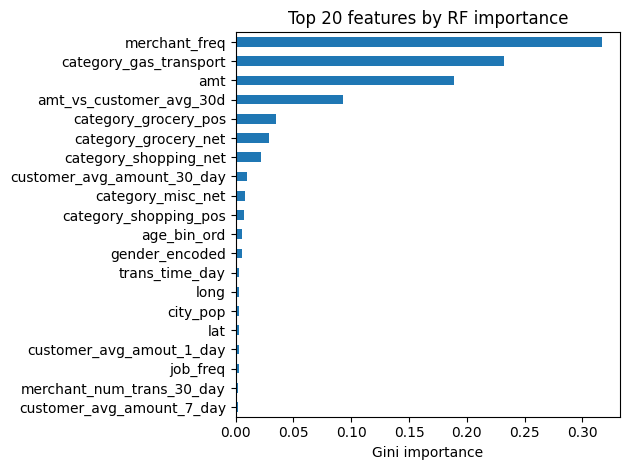
\includegraphics[width=\textwidth]{notebook/cell_62_img_01.png}
        \end{column}
        \begin{column}{0.46\textwidth}
            \textbf{Top RF importance}
            \begin{table}
                \centering
                \tiny
                \begin{tabular}{lr}
                    \toprule
                    \textbf{Feature} & \textbf{Importance} \\
                    \midrule
                    merchant\_freq & 0.3166 \\
                    category\_gas\_transport & 0.2321 \\
                    amt & 0.1885 \\
                    amt\_vs\_customer\_avg\_30d & 0.0926 \\
                    category\_grocery\_pos & 0.0349 \\
                    category\_grocery\_net & 0.0291 \\
                    category\_shopping\_net & 0.0221 \\
                    customer\_avg\_amount\_30\_day & 0.0100 \\
                    \bottomrule
                \end{tabular}
            \end{table}
        \end{column}
    \end{columns}
\end{frame}

\begin{frame}{Feature Selection Rule}
    \textbf{Selection strategy from notebook}:
    \begin{enumerate}
        \item Rank features by Mutual Information.
        \item Rank features by RandomForest importance.
        \item Keep features in top-20 of either ranking.
        \item Remove highly collinear drop candidates.
    \end{enumerate}

    \vspace{0.35cm}
    \begin{table}
        \centering
        \scriptsize
        \begin{tabular}{lll}
            \toprule
            \textbf{Feature 1} & \textbf{Feature 2} & \textbf{Correlation} \\
            \midrule
            category\_gas\_transport & merchant\_freq & 0.9977 \\
            category\_gas\_transport & category\_grocery\_net & 0.9477 \\
            customer\_num\_trans\_1\_day & velocity\_num\_trans\_1d\_30d & 0.9321 \\
            category\_grocery\_net & merchant\_freq & 0.9277 \\
            \bottomrule
        \end{tabular}
    \end{table}
\end{frame}

\begin{frame}{Final Selected Features}
    \textbf{Final result}: 25 selected features from 41 model-ready features.

    \vspace{0.2cm}
    \scriptsize
    \begin{columns}[onlytextwidth]
        \begin{column}{0.5\textwidth}
            \begin{itemize}
                \item age\_bin\_ord
                \item amt
                \item amt\_vs\_customer\_avg\_30d
                \item category\_grocery\_pos
                \item category\_misc\_net
                \item category\_shopping\_net
                \item category\_shopping\_pos
                \item city\_pop
                \item customer\_avg\_amount\_30\_day
                \item customer\_avg\_amount\_7\_day
                \item customer\_avg\_amout\_1\_day
                \item customer\_num\_trans\_30\_day
                \item customer\_num\_trans\_7\_day
            \end{itemize}
        \end{column}
        \begin{column}{0.5\textwidth}
            \begin{itemize}
                \item gender\_encoded
                \item job\_freq
                \item lat
                \item long
                \item merchant\_freq
                \item merchant\_num\_trans\_30\_day
                \item merchant\_risk\_1\_day
                \item merchant\_risk\_30\_day
                \item merchant\_risk\_7\_day
                \item trans\_date\_is\_weekend
                \item trans\_time\_day
                \item trans\_time\_is\_night
            \end{itemize}
        \end{column}
    \end{columns}
\end{frame}

\begin{frame}{Sanity Check: Feature Selection Impact}
    \begin{table}
        \centering
        \small
        \begin{tabular}{lrr}
            \toprule
            \textbf{Feature set} & \textbf{Number of features} & \textbf{Test PR-AUC} \\
            \midrule
            All features & 41 & 0.9588 \\
            Selected features & 25 & 0.9576 \\
            \midrule
            Delta & -16 features & -0.0013 \\
            \bottomrule
        \end{tabular}
    \end{table}

    \vspace{0.3cm}
    \begin{itemize}
        \item Feature selection removes 39\% of features with almost no PR-AUC loss.
        \item Smaller feature set reduces overfitting risk and speeds up XGBoost tuning.
        \item Selected features are used for all final XGBoost experiments.
    \end{itemize}
\end{frame}

\section{Modeling Method}

\begin{frame}{Modeling Approach}
    \begin{columns}
        \begin{column}{0.5\textwidth}
            \textbf{Models}
            \begin{itemize}
                \item \texttt{xgb\_class\_weight}
                \item \texttt{xgb\_undersample}
                \item Both use tuned XGBoost parameters from Optuna.
            \end{itemize}
        \end{column}
        \begin{column}{0.5\textwidth}
            \textbf{Imbalance handling}
            \begin{itemize}
                \item Class weight: keep all data and use \texttt{scale\_pos\_weight}.
                \item Undersampling: majority class reduced to 10:1.
                \item Main model choice: \texttt{xgb\_class\_weight}.
            \end{itemize}
        \end{column}
    \end{columns}

    \vspace{0.4cm}
    \textbf{Reason}: Class weighting keeps the original data distribution and was more stable across chunks.
\end{frame}

\begin{frame}{Baseline Strategy Comparison on Chunk 01}
    \begin{table}
        \centering
        \scriptsize
        \begin{tabular}{llrr}
            \toprule
            \textbf{Name} & \textbf{Strategy} & \textbf{Train size} & \textbf{Val PR-AUC} \\
            \midrule
            rf\_baseline & baseline & 343,209 & 0.9417 \\
            rf\_class\_weight & class weight & 343,209 & 0.9444 \\
            rf\_undersample & undersample & 39,886 & 0.9587 \\
            xgb\_baseline & baseline & 343,209 & 0.9655 \\
            xgb\_class\_weight & class weight & 343,209 & 0.9655 \\
            xgb\_undersample & undersample & 39,886 & 0.9724 \\
            \bottomrule
        \end{tabular}
    \end{table}

    \vspace{0.25cm}
    \begin{itemize}
        \item XGBoost variants outperform RandomForest variants on validation PR-AUC.
        \item The top two candidates selected for Optuna are \texttt{xgb\_undersample} and \texttt{xgb\_class\_weight}.
    \end{itemize}
\end{frame}

\begin{frame}{Tuned XGBoost Parameters}
    \begin{table}
        \centering
        \scriptsize
        \resizebox{\textwidth}{!}{
        \begin{tabular}{lrrrrrrrrr}
            \toprule
            \textbf{Model} & \textbf{n\_est} & \textbf{depth} & \textbf{lr} & \textbf{subsample} & \textbf{colsample} & \textbf{child} & \textbf{alpha} & \textbf{lambda} & \textbf{gamma} \\
            \midrule
            xgb\_undersample & 150 & 8 & 0.016664 & 0.948150 & 0.781684 & 6 & 0.189588 & 0.007976 & 0.660841 \\
            xgb\_class\_weight & 400 & 6 & 0.015384 & 0.880095 & 0.754347 & 1 & 0.155126 & 0.005929 & 3.799895 \\
            \bottomrule
        \end{tabular}
        }
    \end{table}

    \vspace{0.3cm}
    \textbf{Optimization objective}: maximize validation PR-AUC.
\end{frame}

\begin{frame}{Chunk 01 Final Evaluation}
    \begin{table}
        \centering
        \scriptsize
        \begin{tabular}{lrrrrrr}
            \toprule
            \textbf{Model} & \textbf{Test PR-AUC} & \textbf{Threshold} & \textbf{F1} & \textbf{TN} & \textbf{FP} & \textbf{FN / TP} \\
            \midrule
            xgb\_undersample & 0.9614 & 0.7484 & 0.9564 & 106,356 & 0 & 75 / 823 \\
            xgb\_class\_weight & 0.9623 & 0.9722 & 0.9564 & 106,356 & 0 & 75 / 823 \\
            \bottomrule
        \end{tabular}
    \end{table}

    \vspace{0.25cm}
    \begin{itemize}
        \item Both tuned XGBoost models reach precision 1.0000 and recall 0.9165 for fraud on chunk 01 test.
        \item \texttt{xgb\_class\_weight} has slightly higher PR-AUC and keeps the original training distribution.
        \item This strong chunk-01 performance motivates cross-chunk validation to check generalization.
    \end{itemize}
\end{frame}

\begin{frame}{Precision--Recall Curve on Chunk 01}
    \begin{figure}
        \centering
        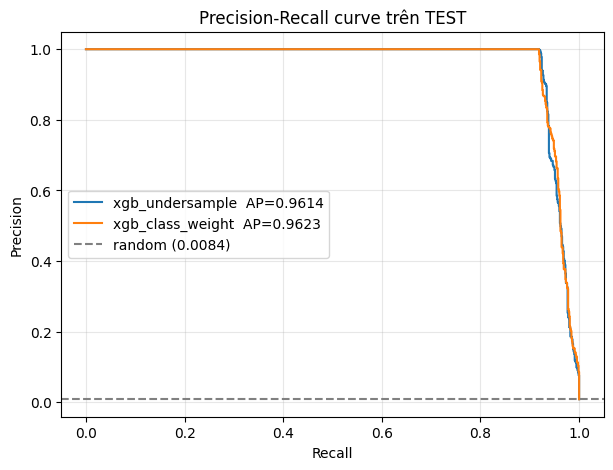
\includegraphics[width=0.72\textwidth]{notebook/cell_88_img_01.png}
        \caption{Precision--Recall curve for the two tuned XGBoost candidates on chunk 01 test set.}
    \end{figure}
\end{frame}

\begin{frame}{Threshold Strategy}
    \textbf{Why threshold matters}:
    \begin{itemize}
        \item PR-AUC measures ranking quality, independent of one fixed threshold.
        \item F1 depends directly on the chosen threshold.
        \item A low F1 can be caused by a bad threshold even if PR-AUC is high.
    \end{itemize}

    \vspace{0.3cm}
    \textbf{Dynamic thresholding}:
    \begin{align}
        \tau^* = \arg\max_{\tau} F1(y_{\text{val}}, \hat{p}_{\text{val}} \ge \tau)
    \end{align}

    \vspace{0.2cm}
    The selected threshold $\tau^*$ is then applied to the final test segment.
\end{frame}

\section{Experiments and Results}

\begin{frame}{Overall Model Comparison}
    \begin{columns}[onlytextwidth, c]
        \begin{column}{0.48\textwidth}
            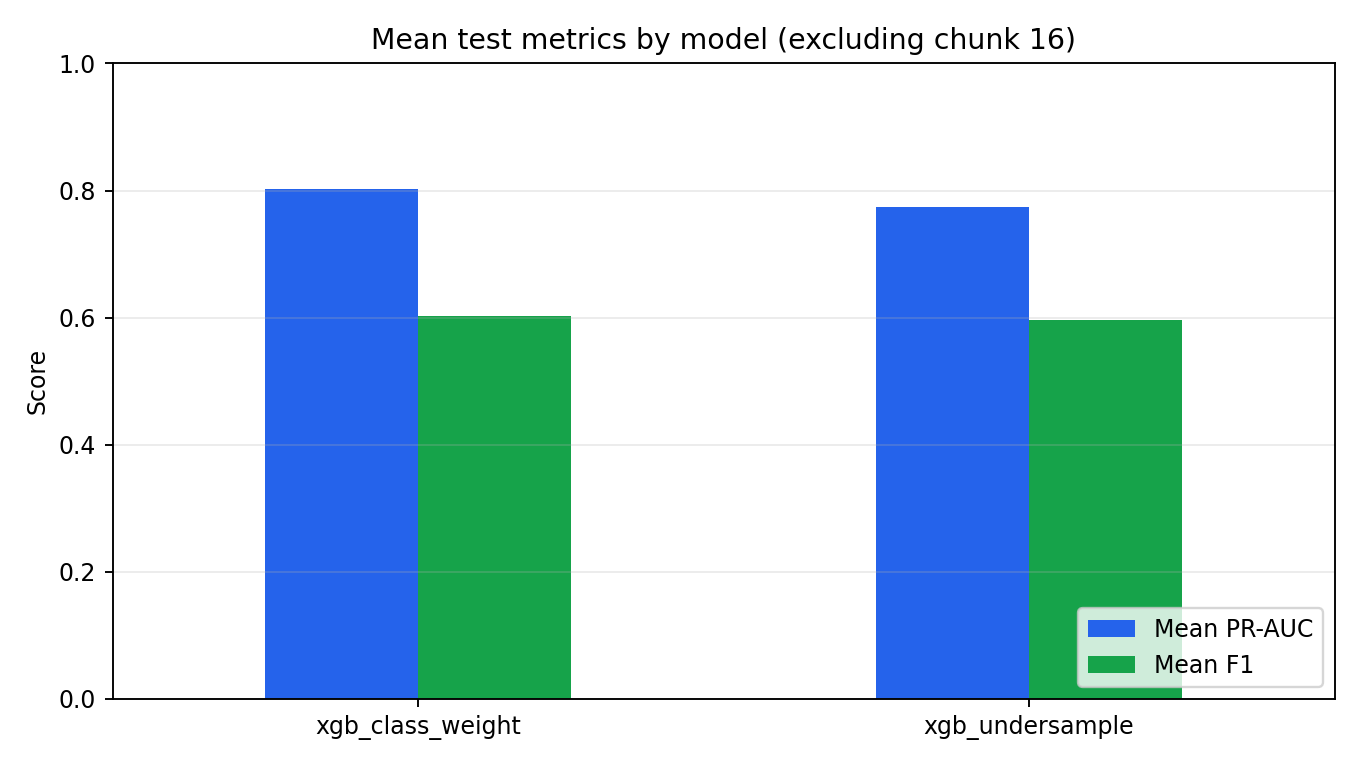
\includegraphics[width=\textwidth]{model_summary_bars.png}
        \end{column}
        \begin{column}{0.5\textwidth}
            \begin{table}
                \centering
                \scriptsize
                \begin{tabular}{lccc}
                    \toprule
                    \textbf{Model} & \textbf{PR-AUC} & \textbf{F1} & \textbf{Best F1 diag.} \\
                    \midrule
                    xgb\_class\_weight & 0.8025 & 0.6031 & 0.7406 \\
                    xgb\_undersample & 0.7736 & 0.5957 & 0.7293 \\
                    \bottomrule
                \end{tabular}
            \end{table}

            \vspace{0.25cm}
            \small
            Values exclude chunk 16 because the test segment has no fraud cases.
        \end{column}
    \end{columns}

    \vspace{0.25cm}
    \textbf{Finding}: \texttt{xgb\_class\_weight} is the better operational baseline.
\end{frame}

\begin{frame}{Chunk-Level Performance}
    \begin{figure}
        \centering
        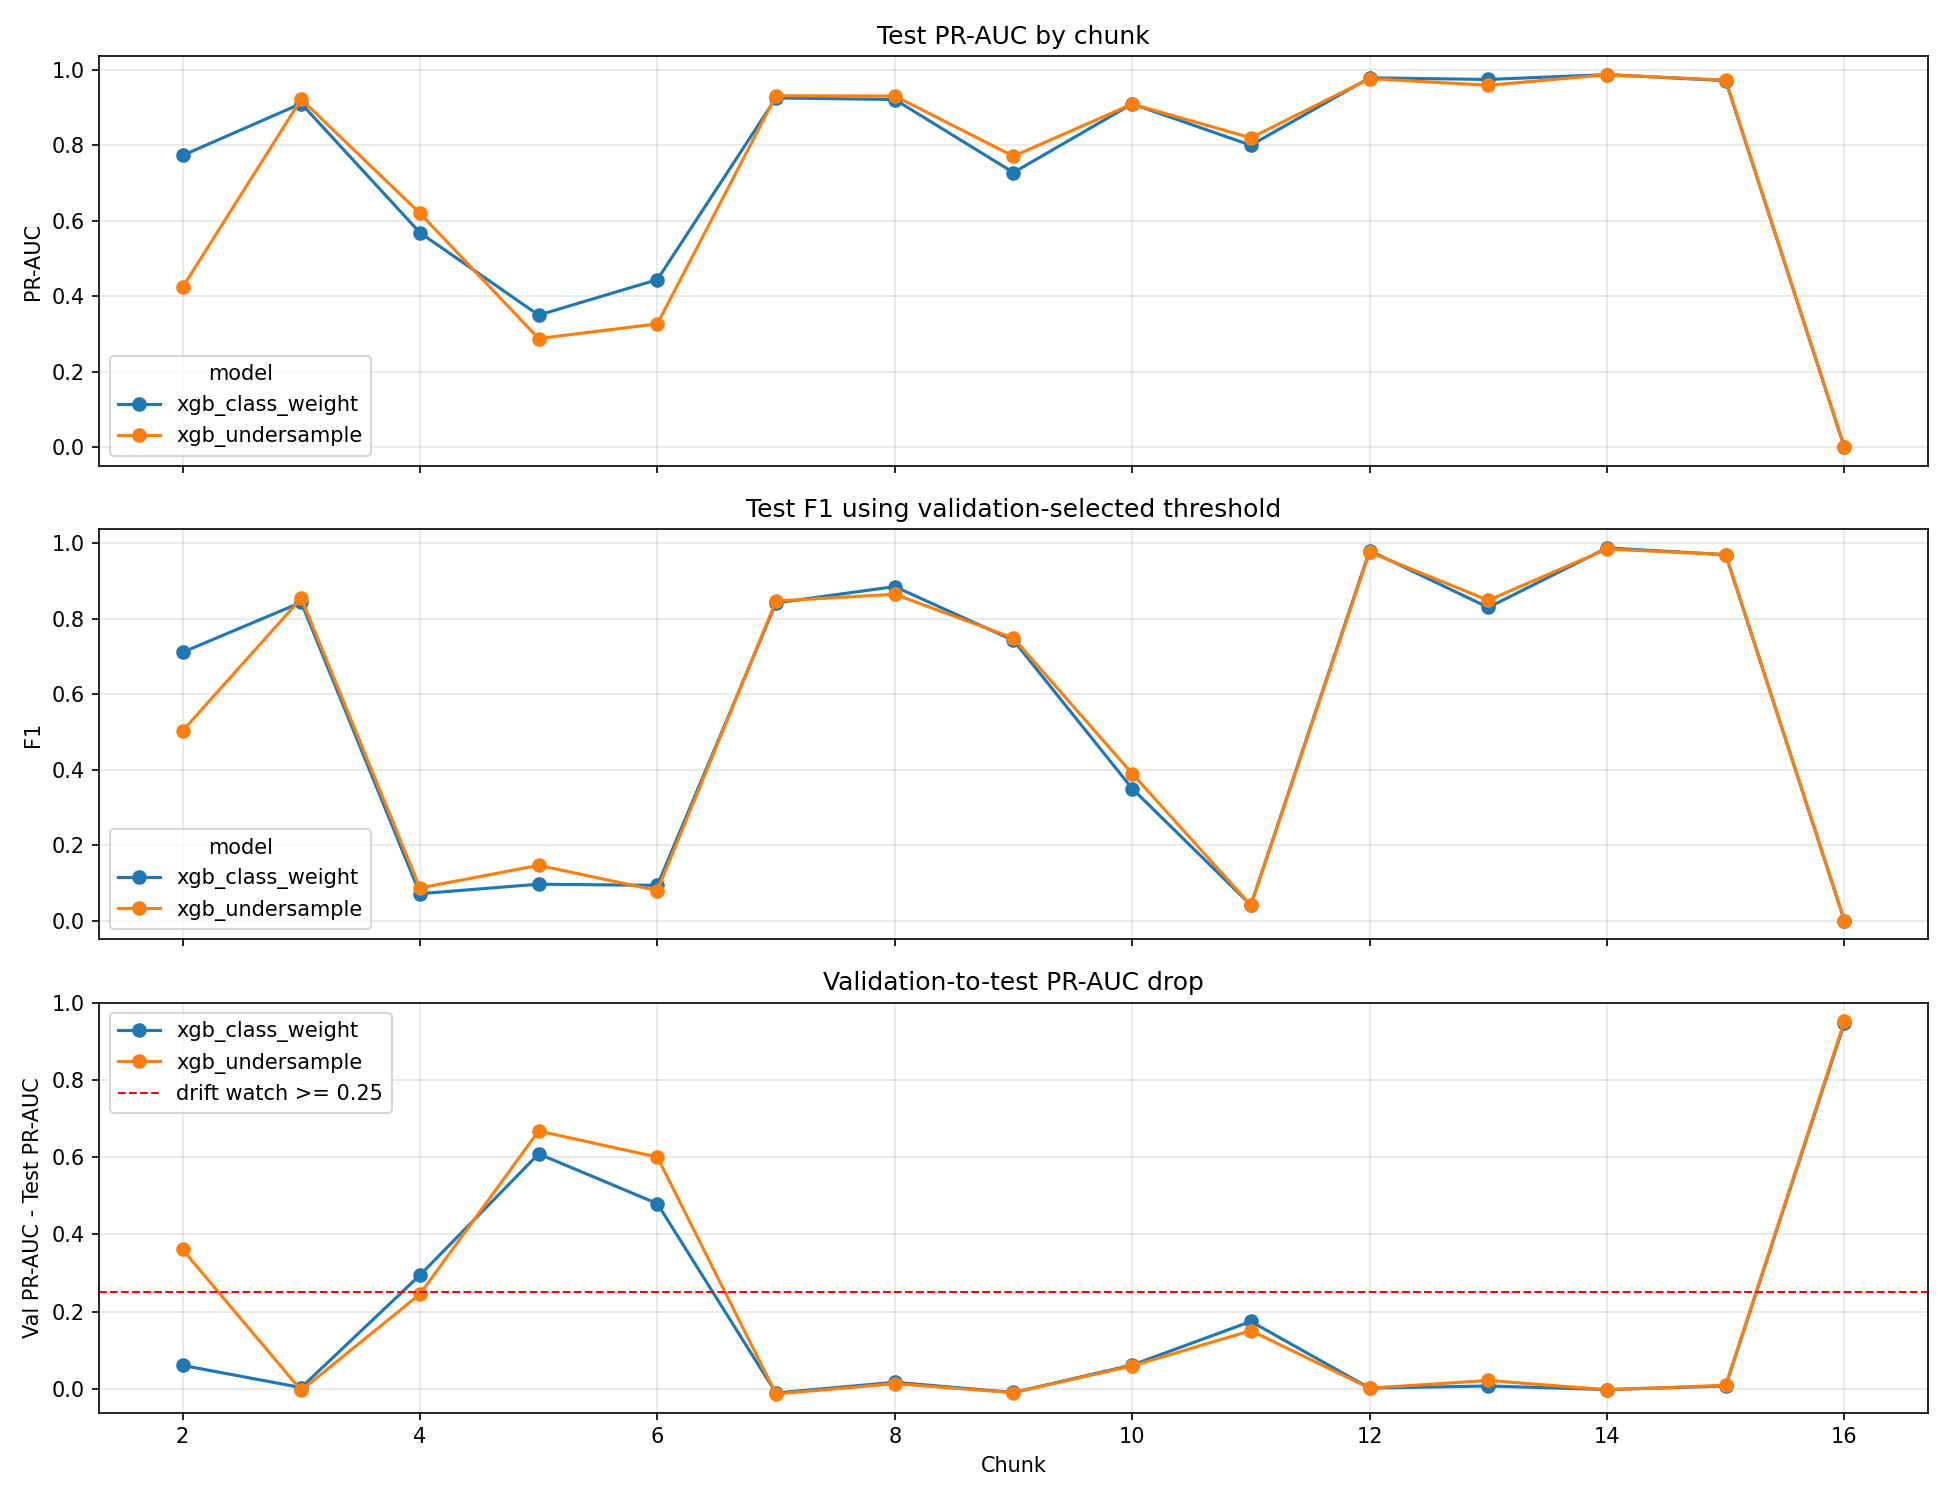
\includegraphics[width=0.95\textwidth]{xgb_chunks_02_16_drift_aware_metrics.png}
        \caption{PR-AUC, F1 and validation-to-test PR-AUC drop across chunks.}
    \end{figure}
\end{frame}

\begin{frame}{Problem Chunks}
    \begin{table}
        \centering
        \tiny
        \resizebox{\textwidth}{!}{
        \begin{tabular}{crrrl}
            \toprule
            \textbf{Chunk} & \textbf{Test PR-AUC} & \textbf{F1 @ Val Th.} & \textbf{Best F1 diag.} & \textbf{Diagnosis} \\
            \midrule
            2 & 0.7726 & 0.7109 & 0.7365 & OK \\
            4 & 0.5682 & 0.0715 & 0.5996 & Ranking drift suspected \\
            5 & 0.3500 & 0.0966 & 0.3905 & Concept/label drift likely \\
            6 & 0.4439 & 0.0935 & 0.4757 & Concept/label drift likely \\
            9 & 0.7274 & 0.7427 & 0.7435 & OK \\
            10 & 0.9091 & 0.3500 & 0.8957 & Threshold calibration drift \\
            11 & 0.7997 & 0.0414 & 0.7559 & Threshold calibration drift \\
            \bottomrule
        \end{tabular}
        }
        \caption{Diagnosis for selected low-F1 chunks using \texttt{xgb\_class\_weight}.}
    \end{table}

    \vspace{0.2cm}
    \textbf{Key point}: Low F1 alone is not enough to conclude concept drift.
\end{frame}

\section{Drift Analysis}

\begin{frame}{Is It Concept Drift?}
    \textbf{Decision rule used in this report}:
    \begin{itemize}
        \item If test PR-AUC drops strongly and best diagnostic F1 remains low:
        \textcolor{red}{concept or label drift is likely}.
        \item If test PR-AUC remains high but F1 is low:
        \textcolor{blue}{threshold/calibration drift is more likely}.
        \item If test set has no positive class:
        do not use that chunk for model-quality conclusion.
    \end{itemize}

    \vspace{0.35cm}
    \textbf{Interpretation}: We separate ranking failure from threshold failure to avoid unnecessary retraining.
\end{frame}

\begin{frame}{Concept or Label Drift Candidates}
    \textbf{Chunks 5 and 6 are the strongest drift candidates.}

    \vspace{0.3cm}
    \begin{itemize}
        \item Chunk 5: validation PR-AUC = 0.9586, test PR-AUC = 0.3500.
        \item Chunk 6: validation PR-AUC = 0.9238, test PR-AUC = 0.4439.
        \item Best diagnostic F1 remains low: 0.3905 and 0.4757.
        \item This means the model no longer ranks fraud well in the test segment.
    \end{itemize}

    \vspace{0.35cm}
    \textbf{Action}: Inspect feature distribution and label pattern, then retrain with a more recent rolling window.
\end{frame}

\begin{frame}{Threshold Calibration Drift}
    \textbf{Chunks 10 and 11 are mainly threshold problems.}

    \vspace{0.3cm}
    \begin{table}
        \centering
        \scriptsize
        \begin{tabular}{crrr}
            \toprule
            \textbf{Chunk} & \textbf{Test PR-AUC} & \textbf{F1 @ Val Th.} & \textbf{Best F1 diag.} \\
            \midrule
            10 & 0.9091 & 0.3500 & 0.8957 \\
            11 & 0.7997 & 0.0414 & 0.7559 \\
            \bottomrule
        \end{tabular}
    \end{table}

    \vspace{0.3cm}
    \textbf{Conclusion}: The ranking is still strong, but the validation threshold is no longer suitable for the test distribution.
\end{frame}

\begin{frame}{Issue Type Distribution}
    \begin{figure}
        \centering
        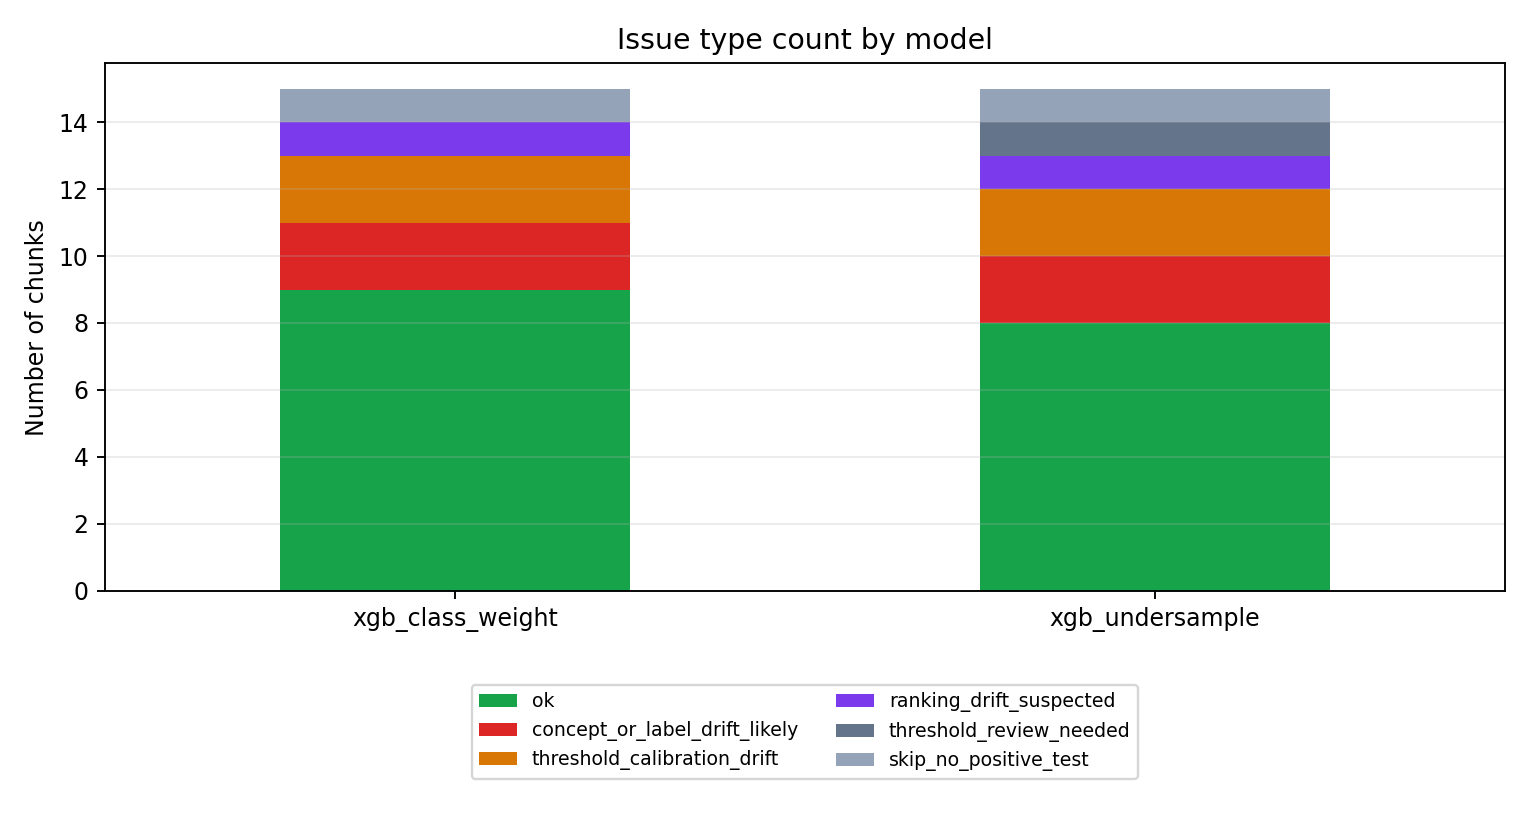
\includegraphics[width=0.88\textwidth]{issue_type_counts.png}
        \caption{Issue categories by model across chunks 02--16.}
    \end{figure}
\end{frame}

\begin{frame}{Validation-to-Test PR-AUC Drop}
    \begin{figure}
        \centering
        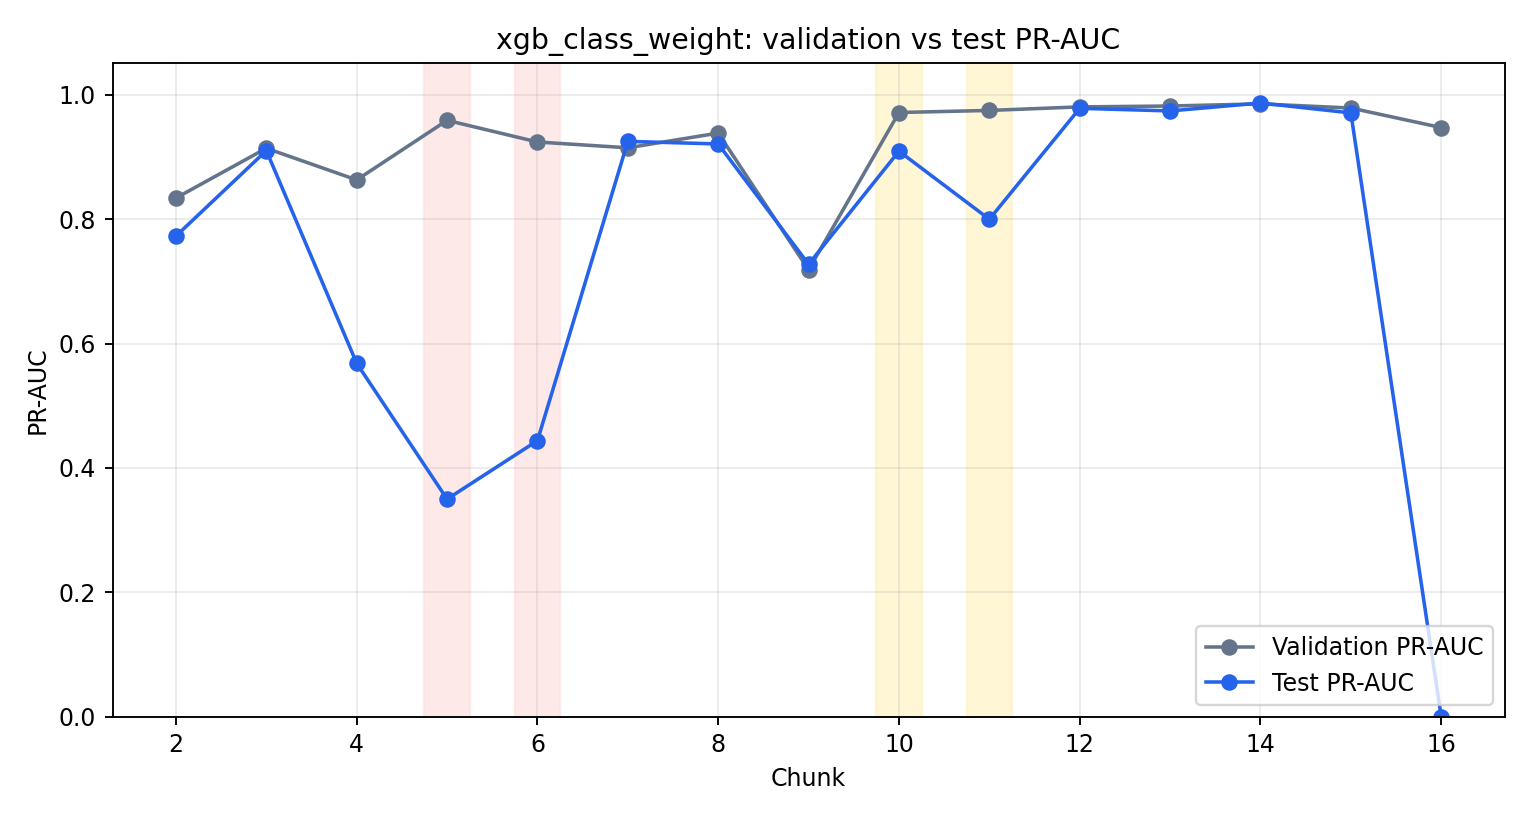
\includegraphics[width=0.9\textwidth]{class_weight_val_test_pr_auc.png}
        \caption{\texttt{xgb\_class\_weight}: comparison between validation and test PR-AUC.}
    \end{figure}
\end{frame}

\section{Conclusion}

\begin{frame}{Recommended Solution}
    \textbf{Best practical strategy}:
    \begin{enumerate}
        \item Use \texttt{xgb\_class\_weight} as the production baseline.
        \item Use dynamic thresholding from the most recent validation window.
        \item Use walk-forward validation instead of random split.
        \item Retrain only when PR-AUC/ranking quality drops, not merely when F1 drops.
        \item Monitor drift using PSI/KS on key features and fraud rate.
    \end{enumerate}

    \vspace{0.3cm}
    \textbf{Reason}: This separates concept drift from threshold drift and avoids unnecessary retraining.
\end{frame}

\begin{frame}{Deployment and Monitoring Plan}
    \begin{columns}
        \begin{column}{0.5\textwidth}
            \textbf{Saved artifacts}
            \begin{itemize}
                \item XGBoost model artifact
                \item Feature order metadata
                \item Threshold policy
                \item Training-window information
            \end{itemize}
        \end{column}
        \begin{column}{0.5\textwidth}
            \textbf{Monitoring}
            \begin{itemize}
                \item PR-AUC and F1 by time chunk
                \item Fraud rate shift
                \item Feature PSI/KS
                \item Separate threshold drift vs concept drift alerts
            \end{itemize}
        \end{column}
    \end{columns}
\end{frame}

\begin{frame}{Conclusions}
    \textbf{Summary}:
    \begin{itemize}
        \item XGBoost is a strong baseline for tabular fraud detection.
        \item \texttt{xgb\_class\_weight} performs better and is more stable than undersampling.
        \item Chunks 5--6 are likely concept/label drift candidates.
        \item Chunks 10--11 mainly show threshold calibration drift.
        \item F1 should always be interpreted together with PR-AUC and threshold diagnostics.
    \end{itemize}

    \vspace{0.4cm}
    \textbf{Final takeaway}: A drift-aware pipeline should combine ranking monitoring, dynamic thresholding, and rolling retraining.
\end{frame}

\begin{frame}
    \centering
    \Huge Thank You!

    \vspace{1cm}

    \Large Questions \& Discussion
\end{frame}

\end{document}
